\documentclass[10pt]{article}
\usepackage[polish]{babel}
\usepackage[utf8]{inputenc}
\usepackage[T1]{fontenc}
\usepackage{amsmath}
\usepackage{amsfonts}
\usepackage{amssymb}
\usepackage[version=4]{mhchem}
\usepackage{stmaryrd}
\usepackage{graphicx}
\usepackage[export]{adjustbox}
\graphicspath{ {./images/} }
\usepackage{bbold}
\usepackage{multirow}

\title{Egzamin maturalny }

\author{}
\date{}


\begin{document}
\maketitle
CENTRALNA\\
KOMISJA\\
EGZAMINACYJNA\\
WYPEŁNIA ZDAJĄCY

\begin{center}
\begin{tabular}{l}
KOD \\
\begin{tabular}{|l|l|}
\hline
\end{tabular} \\
\hline
\end{tabular}
\end{center}\(\quad\)\begin{tabular}{|l|l|l|l|l|l|l|l|l|}
\hline
 &  &  \\
\hline
\end{tabular}

\section*{Miejsce na naklejkę.}
Sprawdź, czy kod na naklejce to E-100.

Jeżeli tak - przyklej naklejkę. Jeżeli nie - zgłoś to nauczycielowi.

\section*{MATEMATYKA}
\section*{Poziom podstawowy}
Symbol arkusza\\
EMAP-PO-100-2405\\
WYPEŁNIA ZESPÓŁ NADZORUJĄCY\\
Uprawnienia zdającego do:\\
dostosowania zasad oceniania dostosowania w zw. z dyskalkulią\\
nieprzenoszenia odpowiedzi na kartę.

\section*{DATA: 8 maja 2024 r. \\
 GoDzINA RozpoczECIA: 9:00 \\
 CZAS trWANIA: \(\mathbf{1 7 0}\) minut}
\section*{46}
Przed rozpoczęciem pracy z arkuszem egzaminacyjnym

\begin{enumerate}
  \item Sprawdź, czy nauczyciel przekazał Ci właściwy arkusz egzaminacyjny, tj. arkusz we właściwej formule, z właściwego przedmiotu na właściwym poziomie.
  \item Jeżeli przekazano Ci niewłaściwy arkusz - natychmiast zgłoś to nauczycielowi. Nie rozrywaj banderol.
  \item Jeżeli przekazano Ci właściwy arkusz - rozerwij banderole po otrzymaniu takiego polecenia od nauczyciela. Zapoznaj się z instrukcją na stronie 2.
\end{enumerate}

\section*{Instrukcja dla zdającego}
\begin{enumerate}
  \item Sprawdź, czy arkusz egzaminacyjny zawiera 31 stron (zadania 1-36). Ewentualny brak zgłoś przewodniczącemu zespołu nadzorującego egzamin.
  \item Na pierwszej stronie arkusza oraz na karcie odpowiedzi wpisz swój numer PESEL i przyklej naklejkę z kodem.
  \item Odpowiedzi do zadań zamkniętych (1-29) zaznacz na karcie odpowiedzi w części karty przeznaczonej dla zdającego. Zamaluj \(\square\) pola do tego przeznaczone. Błędne zaznaczenie otocz kółkiem ( i zaznacz właściwe.
  \item Pamiętaj, że pominięcie argumentacji lub istotnych obliczeń w rozwiązaniu zadania otwartego (30-36) może spowodować, że za to rozwiązanie nie otrzymasz pełnej liczby punktów.
  \item Rozwiązania zadań i odpowiedzi wpisuj w miejscu na to przeznaczonym.
  \item Pisz czytelnie i używaj tylko długopisu lub pióra z czarnym tuszem lub atramentem.
  \item Nie używaj korektora, a błędne zapisy wyraźnie przekreśl.
  \item Nie wpisuj żadnych znaków w części przeznaczonej dla egzaminatora.
  \item Pamiętaj, że zapisy w brudnopisie nie będą oceniane.
  \item Możesz korzystać z Wybranych wzorów matematycznych, cyrkla i linijki oraz kalkulatora prostego. Upewnij się, czy przekazano Ci broszurę z okładką taką jak widoczna poniżej.\\
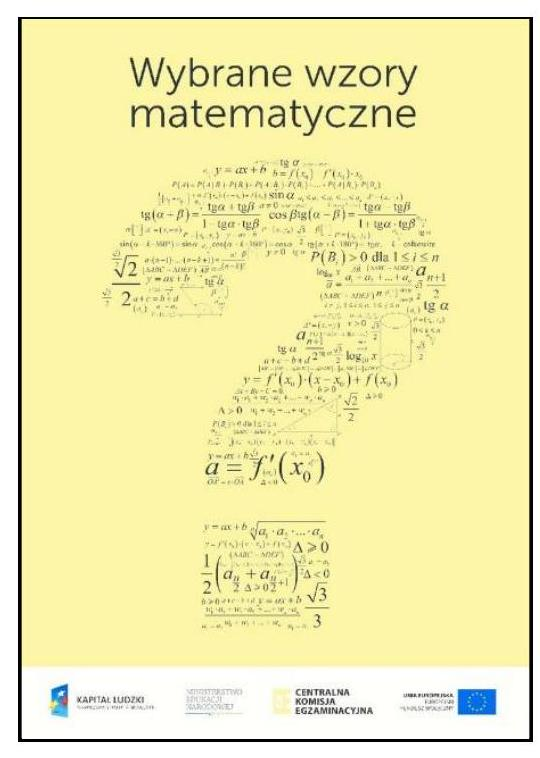
\includegraphics[max width=\textwidth, center]{2024_11_21_0a35d272448d5080a489g-02}
\end{enumerate}

\section*{Zadania egzaminacyjne są wydrukowane na następnych stronach.}
W każdym z zadań od 1. do 29. wybierz i zaznacz na karcie odpowiedzi poprawną odpowiedź.

\section*{Zadanie 1. (0-1)}
Na początku sezonu letniego cenę \(x\) pary sandałów podwyższono o 20\%. Po miesiącu nową cenę obniżono o 10\%. Po obu tych zmianach ta para sandałów kosztowała 81 zł. Początkowa cena \(x\) pary sandałów była równa\\
A. \(45 \mathrm{zł}\)\\
B. \(73,63 \mathrm{zł}\)\\
C. \(75 \mathrm{zł}\)\\
D. \(87,48 \mathrm{zł}\)

\section*{Zadanie 2. (0-1)}
Liczba \(\left(\frac{1}{16}\right)^{8} \cdot 8^{16}\) jest równa\\
A. \(2^{24}\)\\
B. \(2^{16}\)\\
C. \(2^{12}\)\\
D. \(2^{8}\)

\section*{Zadanie 3. (0-1)}
Liczba \(\log _{\sqrt{3}} 9\) jest równa\\
A. 2\\
B. 3\\
C. 4\\
D. 9

\section*{Zadanie 4. (0-1)}
Dla każdej liczby rzeczywistej \(a\) i dla każdej liczby rzeczywistej \(b\) wartość wyrażenia \((2 a+b)^{2}-(2 a-b)^{2}\) jest równa wartości wyrażenia\\
A. \(8 a^{2}\)\\
B. \(8 a b\)\\
C. \(-8 a b\)\\
D. \(2 b^{2}\)

\section*{Zadanie 5. (0-1)}
Zbiorem wszystkich rozwiązań nierówności

\[
1-\frac{3}{2} x<\frac{2}{3}-x
\]

jest przedział\\
A. \(\left(-\infty,-\frac{2}{3}\right)\)\\
B. \(\left(-\infty, \frac{2}{3}\right)\)\\
C. \(\left(-\frac{2}{3},+\infty\right)\)\\
D. \(\left(\frac{2}{3},+\infty\right)\)

\section*{BRUDNOPIS (nie podlega ocenie)}
\begin{center}

\includegraphics[max width=\textwidth]{2024_11_21_0a35d272448d5080a489g-05}
\end{center}

\section*{Zadanie 6. (0-1)}
Największą liczbą będącą rozwiązaniem rzeczywistym równania \(x(x+2)\left(x^{2}+9\right)=0\) jest\\
A. \((-2)\)\\
B. 0\\
C. 2\\
D. 3

\section*{Zadanie 7. (0-1)}
Równanie \(\frac{x+1}{(x+2)(x-3)}=0 \mathrm{w}\) zbiorze liczb rzeczywistych\\
A. nie ma rozwiązania.\\
B. ma dokładnie jedno rozwiązanie: (-1).\\
C. ma dokładnie dwa rozwiązania: (-2) oraz 3.\\
D. ma dokładnie trzy rozwiązania: \((-1),(-2)\) oraz 3.

\section*{Zadanie 8. (0-1)}
W październiku 2022 roku założono dwa sady, w których posadzono łącznie 1960 drzew. Po roku stwierdzono, że uschło 5\% drzew w pierwszym sadzie i 10\% drzew w drugim sadzie. Uschnięte drzewa usunięto, a nowych nie dosadzano.\\
Liczba drzew, które pozostały w drugim sadzie, stanowiła \(60 \%\) liczby drzew, które pozostały w pierwszym sadzie.\\
Niech \(x\) oraz \(y\) oznaczają liczby drzew posadzonych - odpowiednio - w pierwszym i drugim sadzie.

Układem równań, którego poprawne rozwiązanie prowadzi do obliczenia liczby \(x\) drzew posadzonych w pierwszym sadzie oraz liczby \(y\) drzew posadzonych w drugim sadzie, jest\\
A. \(\left\{\begin{array}{l}x+y=1960 \\ 0,6 \cdot 0,95 x=0,9 y\end{array}\right.\)\\
B. \(\left\{\begin{array}{l}x+y=1960 \\ 0,95 x=0,6 \cdot 0,9 y\end{array}\right.\)\\
C. \(\left\{\begin{array}{l}x+y=1960 \\ 0,05 x=0,6 \cdot 0,1 y\end{array}\right.\)\\
D. \(\left\{\begin{array}{l}x+y=1960 \\ 0,4 \cdot 0,95 x=0,9 y\end{array}\right.\)

BRUDNOPIS (nie podlega ocenie)\\

\includegraphics[max width=\textwidth, center]{2024_11_21_0a35d272448d5080a489g-07}

Średnia arytmetyczna trzech liczb: \(a, b, c\), jest równa 9.\\
Średnia arytmetyczna sześciu liczb: \(a, a, b, b, c, c\), jest równa\\
A. 9\\
B. 6\\
C. 4,5\\
D. 18

\section*{Zadanie 10. (0-1)}
Na rysunku przedstawiono dwie proste równoległe, które są interpretacją geometryczną jednego z poniższych układów równań A-D.\\
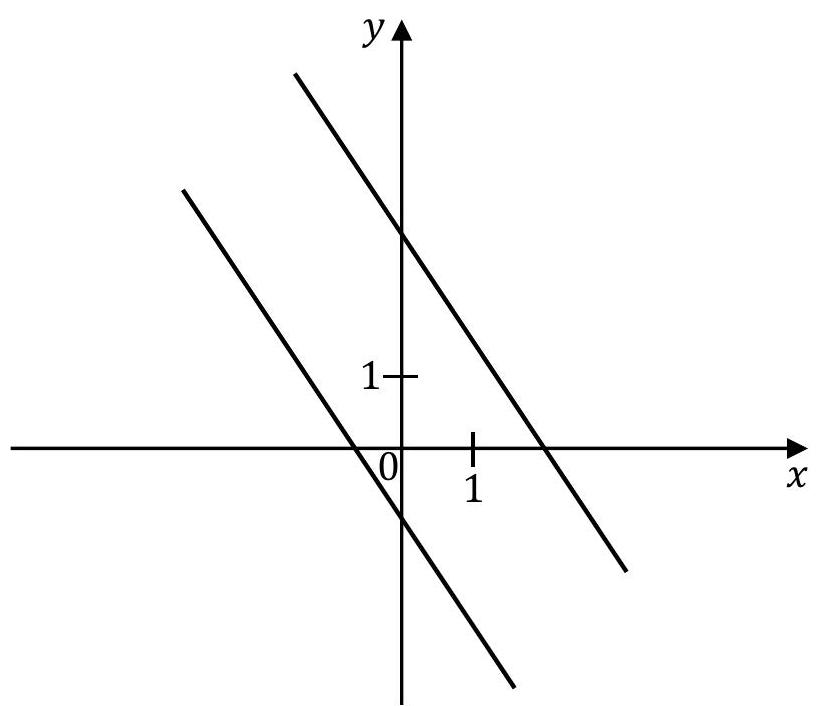
\includegraphics[max width=\textwidth, center]{2024_11_21_0a35d272448d5080a489g-08}

Układem równań, którego interpretację geometryczną przedstawiono na rysunku, jest\\
A. \(\left\{\begin{array}{l}y=-\frac{3}{2} x+3 \\ y=-\frac{3}{2} x-1\end{array}\right.\)\\
B. \(\left\{\begin{array}{l}y=\frac{3}{2} x+3 \\ y=-\frac{2}{3} x-1\end{array}\right.\)\\
C. \(\left\{\begin{array}{l}y=\frac{3}{2} x+3 \\ y=\frac{3}{2} x-1\end{array}\right.\)\\
D. \(\left\{\begin{array}{l}y=-\frac{3}{2} x-3 \\ y=\frac{3}{2} x+1\end{array}\right.\)

BRUDNOPIS (nie podlega ocenie)\\

\includegraphics[max width=\textwidth, center]{2024_11_21_0a35d272448d5080a489g-09}

\section*{Zadanie 11. (0-1)}
Na rysunku przedstawiono wykres funkcji \(f\).\\
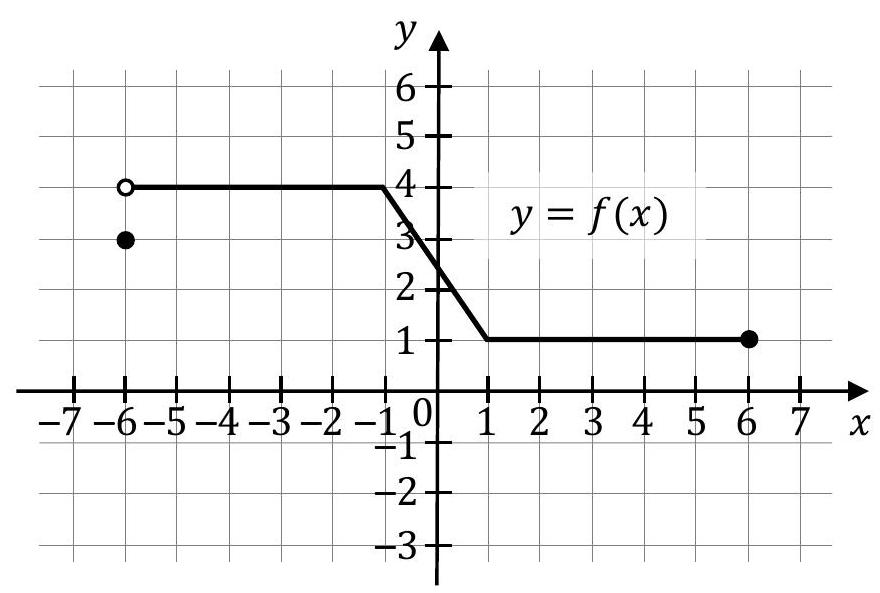
\includegraphics[max width=\textwidth, center]{2024_11_21_0a35d272448d5080a489g-10}

Zbiorem wartości tej funkcji jest\\
A. \((-6,6)\)\\
B. \((1,4)\)\\
C. \(\langle 1,4\rangle\)\\
D. \(\langle-6,6\rangle\)

\section*{Zadanie 12. (0-1)}
Funkcja liniowa \(f\) jest określona wzorem \(f(x)=(-2 k+3) x+k-1\), gdzie \(k \in \mathbb{R}\).\\
Funkcja \(f\) jest malejąca dla każdej liczby \(k\) należącej do przedziału\\
A. \((-\infty, 1)\)\\
B. \(\left(-\infty,-\frac{3}{2}\right)\)\\
C. \((1,+\infty)\)\\
D. \(\left(\frac{3}{2},+\infty\right)\)

\section*{Zadanie 13. (0-1)}
Funkcje liniowe \(f\) oraz \(g\), określone wzorami \(f(x)=3 x+6\) oraz \(g(x)=a x+7\), mają to samo miejsce zerowe.\\
Współczynnik a we wzorze funkcji \(g\) jest równy\\
A. \(\left(-\frac{7}{2}\right)\)\\
B. \(\left(-\frac{2}{7}\right)\)\\
C. \(\frac{2}{7}\)\\
D. \(\frac{7}{2}\)

BRUDNOPIS (nie podlega ocenie)\\

\includegraphics[max width=\textwidth, center]{2024_11_21_0a35d272448d5080a489g-11}

\section*{Informacja do zadań 14.-15.}
Na rysunku przedstawiono fragment paraboli, która jest wykresem funkcji kwadratowej \(f\) (zobacz rysunek). Wierzchołek tej paraboli oraz punkty przecięcia paraboli z osiami układu współrzędnych mają obie współrzędne całkowite.\\
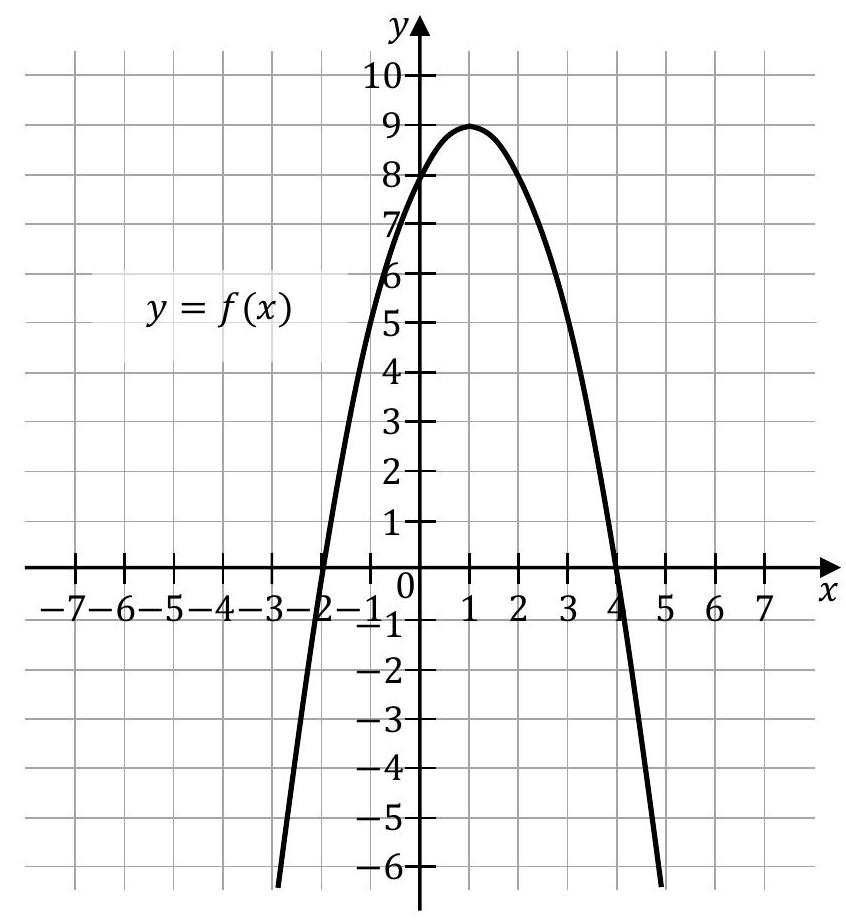
\includegraphics[max width=\textwidth, center]{2024_11_21_0a35d272448d5080a489g-12}

\section*{Zadanie 14. (0-1)}
Funkcja kwadratowa \(f\) jest określona wzorem\\
A. \(f(x)=-(x+1)^{2}-9\)\\
B. \(f(x)=-(x-1)^{2}+9\)\\
C. \(f(x)=-(x-1)^{2}-9\)\\
D. \(f(x)=-(x+1)^{2}+9\)

\section*{Zadanie 15. (0-1)}
Dla funkcji \(f\) prawdziwa jest równość\\
A. \(f(-4)=f(6)\)\\
B. \(f(-4)=f(4)\)\\
C. \(f(-4)=f(5)\)\\
D. \(f(-4)=f(7)\)

BRUDNOPIS (nie podlega ocenie)\\

\includegraphics[max width=\textwidth, center]{2024_11_21_0a35d272448d5080a489g-13}

\section*{Zadanie 16. (0-1)}
W ciągu arytmetycznym \(\left(a_{n}\right)\), określonym dla każdej liczby naturalnej \(n \geq 1\), dane są wyrazy \(a_{4}=-2\) oraz \(a_{6}=16\).\\
Piąty wyraz tego ciągu jest równy\\
A. \(\frac{7}{2}\)\\
B. \(\frac{9}{2}\)\\
C. 7\\
D. 9

\section*{Zadanie 17. (0-1)}
Ciąg geometryczny \(\left(a_{n}\right)\) jest określony wzorem \(a_{n}=2^{n-1}\), dla każdej liczby naturalnej \(n \geq 1\). lloraz tego ciągu jest równy\\
A. \(\frac{1}{2}\)\\
B. \((-2)\)\\
C. 2\\
D. 1

\section*{Zadanie 18. (0-1)}
Ciąg \(\left(b_{n}\right)\) jest określony wzorem \(b_{n}=(n+2)(7-n)\), dla każdej liczby naturalnej \(n \geq 1\). Liczba dodatnich wyrazów ciągu \(\left(b_{n}\right)\) jest równa\\
A. 6\\
B. 7\\
C. 8\\
D. 9

\section*{Zadanie 19. (0-1)}
Liczba \(\sin ^{3} 20^{\circ}+\cos ^{2} 20^{\circ} \cdot \sin 20^{\circ}\) jest równa\\
A. \(\cos 20^{\circ}\)\\
B. \(\sin 20^{\circ}\)\\
C. \(\operatorname{tg} 20^{\circ}\)\\
D. \(\sin 20^{\circ} \cdot \cos 20^{\circ}\)

\section*{Zadanie 20. (0-1)}
Kąt \(\alpha\) jest ostry oraz \(\cos \alpha=\frac{5}{13}\). Wtedy\\
A. \(\operatorname{tg} \alpha=\frac{12}{13}\)\\
B. \(\operatorname{tg} \alpha=\frac{12}{5}\)\\
C. \(\operatorname{tg} \alpha=\frac{5}{12}\)\\
D. \(\operatorname{tg} \alpha=\frac{13}{12}\)

BRUDNOPIS (nie podlega ocenie)\\

\includegraphics[max width=\textwidth, center]{2024_11_21_0a35d272448d5080a489g-15}

\section*{Zadanie 21. (0-1)}
Dany jest równoległobok o bokach długości 3 i 4 oraz o kącie między nimi o mierze \(120^{\circ}\). Pole tego równoległoboku jest równe\\
A. 6\\
B. \(6 \sqrt{3}\)\\
C. 12\\
D. \(12 \sqrt{3}\)

\section*{Zadanie 22. (0-1)}
W trójkącie \(M K C\) bok \(M K\) ma długość 24. Prosta równoległa do boku \(M K\) przecina boki \(M C\) i \(K C\)-odpowiednio - w punktach \(A\) oraz \(B\) takich, że \(|A B|=6\) i \(|A C|=3\) (zobacz rysunek).\\
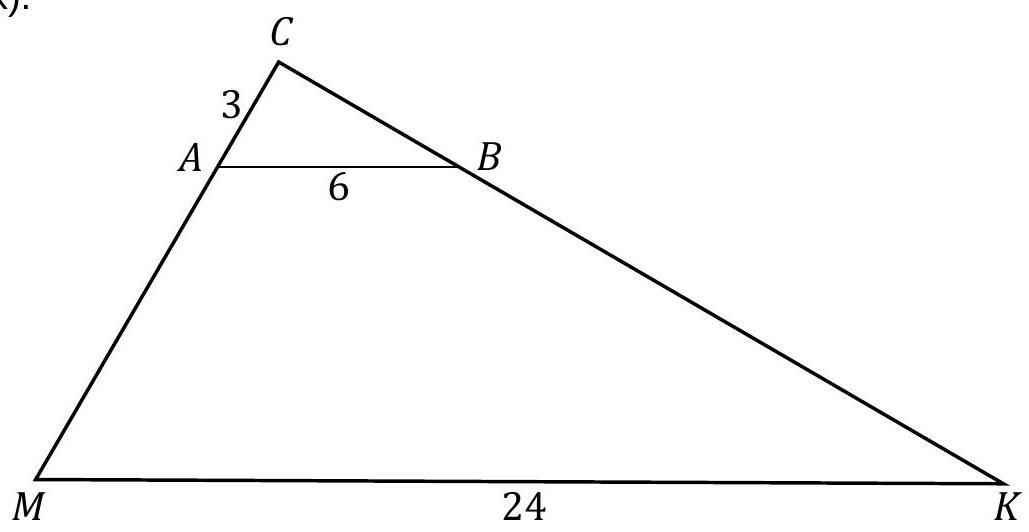
\includegraphics[max width=\textwidth, center]{2024_11_21_0a35d272448d5080a489g-16(1)}

Długość odcinka \(M A\) jest równa\\
A. 18\\
B. 15\\
C. 9\\
D. 12

\section*{Zadanie 23. (0-1)}
W trójkącie \(A B C\), wpisanym w okrąg o środku w punkcie \(S\), kąt \(A C B\) ma miarę \(42^{\circ}\) (zobacz rysunek).\\
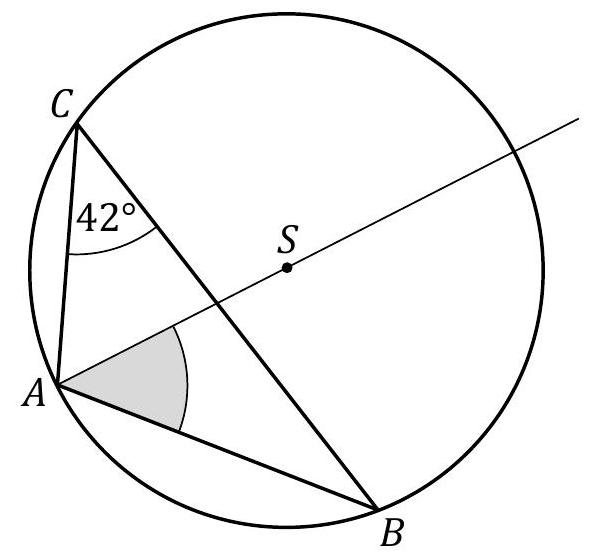
\includegraphics[max width=\textwidth, center]{2024_11_21_0a35d272448d5080a489g-16}

Miara kąta ostrego \(B A S\) jest równa\\
A. \(42^{\circ}\)\\
B. \(45^{\circ}\)\\
C. \(48^{\circ}\)\\
D. \(69^{\circ}\)

BRUDNOPIS (nie podlega ocenie)\\

\includegraphics[max width=\textwidth, center]{2024_11_21_0a35d272448d5080a489g-17}

\section*{Zadanie 24. (0-1)}
Proste \(k\) oraz \(l\) są określone równaniami

\[
\begin{aligned}
& k: y=(m+1) x+7 \\
& l: y=-2 x+7
\end{aligned}
\]

Proste \(k\) oraz \(l\) są prostopadłe, gdy liczba \(m\) jest równa\\
A. \(\left(-\frac{1}{2}\right)\)\\
B. \(\frac{1}{2}\)\\
C. \((-3)\)\\
D. 1

\section*{Zadanie 25. (0-1)}
Na prostej \(l\) o współczynniku kierunkowym \(\frac{1}{2}\) leżą punkty \(A=(2,-4)\) oraz \(B=(0, b)\). Wtedy liczba \(b\) jest równa\\
A. \((-5)\)\\
B. 10\\
C. \((-2)\)\\
D. 0

\section*{Zadanie 26. (0-1)}
Wysokość graniastosłupa prawidłowego sześciokątnego jest równa 6 (zobacz rysunek). Pole podstawy tego graniastosłupa jest równe \(15 \sqrt{3}\).\\
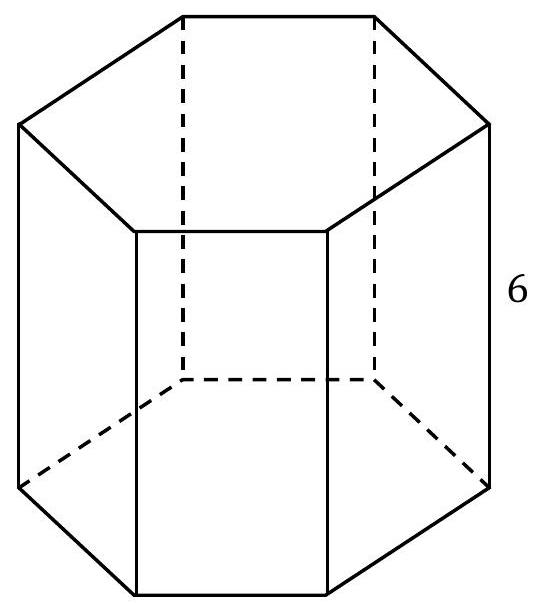
\includegraphics[max width=\textwidth, center]{2024_11_21_0a35d272448d5080a489g-18}

Pole ¡ednej ściany bocznej tego graniastosłupa jest równe\\
A. \(36 \sqrt{10}\)\\
B. 60\\
C. \(6 \sqrt{10}\)\\
D. 360

BRUDNOPIS (nie podlega ocenie)\\

\includegraphics[max width=\textwidth, center]{2024_11_21_0a35d272448d5080a489g-19}

\section*{Zadanie 27. (0-1)}
Kąt nachylenia najdłuższej przekątnej graniastosłupa prawidłowego sześciokątnego do płaszczyzny podstawy jest zaznaczony na rysunku\\
A.\\
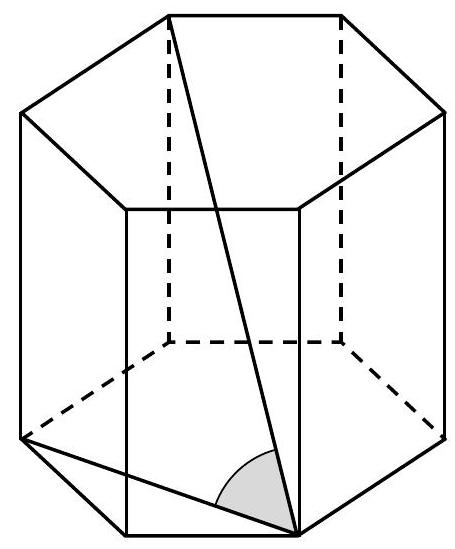
\includegraphics[max width=\textwidth, center]{2024_11_21_0a35d272448d5080a489g-20(2)}\\
B.\\
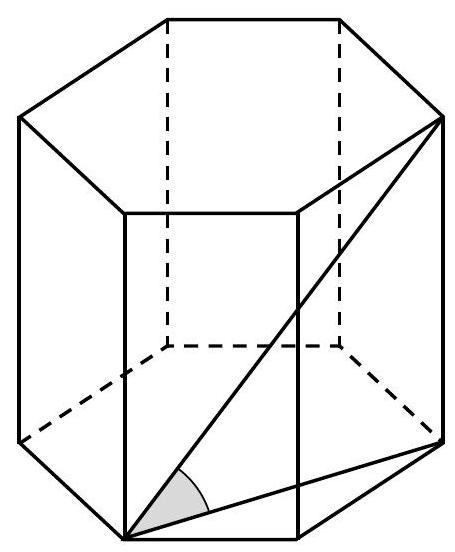
\includegraphics[max width=\textwidth, center]{2024_11_21_0a35d272448d5080a489g-20(1)}\\
C.\\
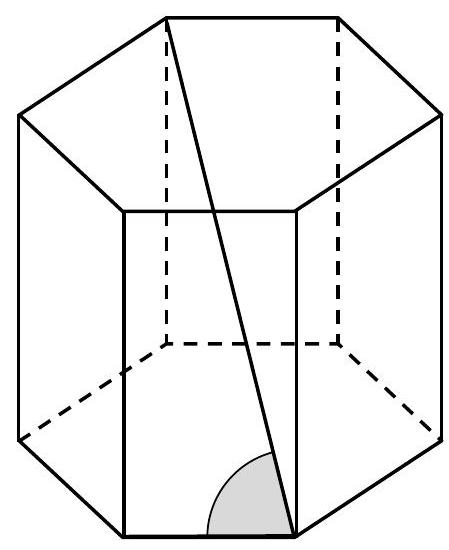
\includegraphics[max width=\textwidth, center]{2024_11_21_0a35d272448d5080a489g-20}\\
D.\\
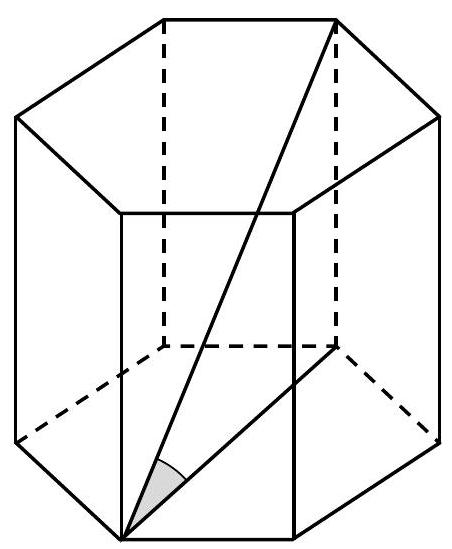
\includegraphics[max width=\textwidth, center]{2024_11_21_0a35d272448d5080a489g-20(3)}

\section*{Zadanie 28. (0-1)}
Objętość ostrosłupa prawidłowego czworokątnego jest równa 64. Wysokość tego ostrosłupa jest równa 12.\\
Długość krawędzi podstawy tego ostrosłupa jest równa\\
A. 2\\
B. 4\\
C. 6\\
D. 8

\section*{Zadanie 29. (0-1)}
Rozważamy wszystkie kody czterocyfrowe utworzone tylko z cyfr 1, 3, 6, 8, przy czym w każdym kodzie każda z tych cyfr występuje dokładnie jeden raz.\\
Liczba wszystkich takich kodów jest równa\\
A. 4\\
B. 10\\
C. 24\\
D. 16

BRUDNOPIS (nie podlega ocenie)\\

\includegraphics[max width=\textwidth, center]{2024_11_21_0a35d272448d5080a489g-21}

Zadanie 30. (0-2)\\
Rozwiąż nierówność

\[
x^{2}-4 \leq 3 x
\]

\begin{center}

\includegraphics[max width=\textwidth]{2024_11_21_0a35d272448d5080a489g-22}
\end{center}

Zadanie 31. (0-2)\\
Wykaż, że dla każdej liczby rzeczywistej \(x\) i dla każdej liczby rzeczywistej \(y\) takich, że \(x \neq y\), prawdziwa jest nierówność

\[
(3 x+y)(x+3 y)>16 x y
\]

\begin{center}

\includegraphics[max width=\textwidth]{2024_11_21_0a35d272448d5080a489g-23}
\end{center}

\begin{center}
\begin{tabular}{|c|l|c|c|}
\hline
\multirow{3}{*}{\begin{tabular}{c}
Wypełnia \\
egzaminator \\
\end{tabular}} & Nr zadania & 30. & 31. \\
\cline { 2 - 4 }
 & Maks. liczba pkt & 2 & 2 \\
\cline { 2 - 4 }
 & Uzyskana liczba pkt &  &  \\
\hline
\end{tabular}
\end{center}

Zadanie 32. (0-2)\\
Osią symetrii wykresu funkcji kwadratowej \(f(x)=x^{2}+b x+c\) jest prosta o równaniu \(x=-2\). Jednym z miejsc zerowych funkcji \(f\) jest liczba 1. Oblicz współczynniki \(b\) oraz \(c\).\\

\includegraphics[max width=\textwidth, center]{2024_11_21_0a35d272448d5080a489g-24}

Zadanie 33. (0-2)\\
Ciąg arytmetyczny \(\left(a_{n}\right)\) jest określony dla każdej liczby naturalnej \(n \geq 1\). Trzeci wyraz tego ciągu jest równy \((-1)\), a suma piętnastu początkowych kolejnych wyrazów tego ciągu jest równa (-165).\\
Oblicz różnicę tego ciągu.\\

\includegraphics[max width=\textwidth, center]{2024_11_21_0a35d272448d5080a489g-25}

\begin{center}
\begin{tabular}{|c|l|c|c|}
\hline
\multirow{2}{*}{\begin{tabular}{c}
Wypełnia \\
egzaminator \\
\end{tabular}} & Nr zadania & 32. & 33. \\
\cline { 2 - 4 }
 & Maks. liczba pkt & 2 & 2 \\
\cline { 2 - 4 }
 & Uzyskana liczba pkt &  &  \\
\hline
\end{tabular}
\end{center}

Zadanie 34. (0-2)\\
Dany jest równoległobok \(A B C D\), w którym \(A=(-2,6)\) oraz \(B=(10,2)\). Przekątne \(A C\) oraz \(B D\) tego równoległoboku przecinają się w punkcie \(P=(6,7)\).\\
Oblicz długość boku \(B C\) tego równoległoboku.\\

\includegraphics[max width=\textwidth, center]{2024_11_21_0a35d272448d5080a489g-26}

Zadanie 35. (0-2)\\
Dany jest pięcioelementowy zbiór \(K=\{5,6,7,8,9\}\). Wylosowanie każdej liczby z tego zbioru jest jednakowo prawdopodobne. Ze zbioru \(K\) losujemy ze zwracaniem kolejno dwa razy po jednej liczbie i zapisujemy je w kolejności losowania.\\
Oblicz prawdopodobieństwo zdarzenia \(A\) polegającego na tym, że suma wylosowanych liczb jest liczbą parzystą.

\begin{center}
\begin{tabular}{|c|c|c|c|c|c|c|c|c|c|c|c|c|c|c|c|c|c|c|c|c|c|c|c|c|c|c|c|c|c|c|}
\hline
 &  &  &  &  &  &  &  &  &  &  &  &  &  &  &  &  &  &  &  &  &  &  &  &  &  &  &  &  &  &  \\
\hline
 &  &  &  &  &  &  &  &  &  &  &  &  &  &  &  &  &  &  &  &  &  &  &  &  &  &  &  &  &  &  \\
\hline
 &  &  &  &  &  &  &  &  &  &  &  &  &  &  &  &  &  &  &  &  &  &  &  &  &  &  &  &  &  &  \\
\hline
 &  &  &  &  &  &  &  &  &  &  &  &  &  &  &  &  &  &  &  &  &  &  &  &  &  &  &  &  &  &  \\
\hline
 &  &  &  &  &  &  &  &  &  &  &  &  &  &  &  &  &  &  &  &  &  &  &  &  &  &  &  &  &  &  \\
\hline
 &  &  &  &  &  &  &  &  &  &  &  &  &  &  &  &  &  &  &  &  &  &  &  &  &  &  &  &  &  &  \\
\hline
 &  &  &  &  &  &  &  &  &  &  &  &  &  &  &  &  &  &  &  &  &  &  &  &  &  &  &  &  &  &  \\
\hline
 &  &  &  &  &  &  &  &  &  &  &  &  &  &  &  &  &  &  &  &  &  &  &  &  &  &  &  &  &  &  \\
\hline
 &  &  &  &  &  &  &  &  &  &  &  &  &  &  &  &  &  &  &  &  &  &  &  &  &  &  &  &  &  &  \\
\hline
 &  &  &  &  &  &  &  &  &  &  &  &  &  &  &  &  &  &  &  &  &  &  &  &  &  &  &  &  &  &  \\
\hline
 &  &  &  &  &  &  &  &  &  &  &  &  &  &  &  &  &  &  &  &  &  &  &  &  &  &  &  &  &  &  \\
\hline
 &  &  &  &  &  &  &  &  &  &  &  &  &  &  &  &  &  &  &  &  &  &  &  &  &  &  &  &  &  &  \\
\hline
 &  &  &  &  &  &  &  &  &  &  &  &  &  &  &  &  &  &  &  &  &  &  &  &  &  &  &  &  &  &  \\
\hline
 &  &  &  &  &  &  &  &  &  &  &  &  &  &  &  &  &  &  &  &  &  &  &  &  &  &  &  &  &  &  \\
\hline
 &  &  &  &  &  &  &  &  &  &  &  &  &  &  &  &  &  &  &  &  &  &  &  &  &  &  &  &  &  &  \\
\hline
 &  &  &  &  &  &  &  &  &  &  &  &  &  &  &  &  &  &  &  &  &  &  &  &  &  &  &  &  &  &  \\
\hline
 &  &  &  &  &  &  &  &  &  &  &  &  &  &  &  &  &  &  &  &  &  &  &  &  &  &  &  &  &  &  \\
\hline
 &  &  &  &  &  &  &  &  &  &  &  &  &  &  &  &  &  &  &  &  &  &  &  &  &  &  &  &  &  &  \\
\hline
 &  &  &  &  &  &  &  &  &  &  &  &  &  &  &  &  &  &  &  &  &  &  &  &  &  &  &  &  &  &  \\
\hline
 &  &  &  &  &  &  &  &  &  &  &  &  &  &  &  &  &  &  &  &  &  &  &  &  &  &  &  &  &  &  \\
\hline
 &  &  &  &  &  &  &  &  &  &  &  &  &  &  &  &  &  &  &  &  &  &  &  &  &  &  &  &  &  &  \\
\hline
 &  &  &  &  &  &  &  &  &  &  &  &  &  &  &  &  &  &  &  &  &  &  &  &  &  &  &  &  &  &  \\
\hline
 &  &  &  &  &  &  &  &  &  &  &  &  &  &  &  &  &  &  &  &  &  &  &  &  &  &  &  &  &  &  \\
\hline
 &  &  &  &  &  &  &  &  &  &  &  &  &  &  &  &  &  &  &  &  &  &  &  &  &  &  &  &  &  &  \\
\hline
 &  &  &  &  &  &  &  &  &  &  &  &  &  &  &  &  &  &  &  &  &  &  &  &  &  &  &  &  &  &  \\
\hline
 &  &  &  &  &  &  &  &  &  &  &  &  &  &  &  &  &  &  &  &  &  &  &  &  &  &  &  &  &  &  \\
\hline
 &  &  &  &  &  &  &  &  &  &  &  &  &  &  &  &  &  &  &  &  &  &  &  &  &  &  &  &  &  &  \\
\hline
 &  &  &  &  &  &  &  &  &  &  &  &  &  &  &  &  &  &  &  &  &  &  &  &  &  &  &  &  &  &  \\
\hline
 &  &  &  &  &  &  &  &  &  &  &  &  &  &  &  &  &  &  &  &  &  &  &  &  &  &  &  &  &  &  \\
\hline
 & \textbackslash  &  &  &  &  &  &  &  &  &  &  &  &  &  &  &  &  &  &  &  &  &  &  &  &  &  &  &  &  &  \\
\hline
 &  &  &  &  &  &  &  &  &  &  &  &  &  &  &  &  &  &  &  &  &  &  &  &  &  &  &  &  &  &  \\
\hline
 &  &  &  &  &  &  &  &  &  &  &  &  &  &  &  &  &  &  &  &  &  &  &  &  &  &  &  &  &  &  \\
\hline
 & \textbackslash  &  &  &  &  &  &  &  &  &  &  &  &  &  &  &  &  &  &  &  &  &  &  &  &  &  &  &  &  &  \\
\hline
 & \textbackslash  &  &  &  &  &  &  &  &  &  &  &  &  &  &  &  &  &  &  &  &  &  &  &  &  &  &  &  &  &  \\
\hline
 & - &  &  &  &  &  &  &  &  &  &  &  &  &  &  &  &  &  &  &  &  &  &  &  &  &  &  &  &  &  \\
\hline
 & \textbackslash  &  &  &  &  &  &  &  &  &  &  &  &  &  &  &  &  &  &  &  &  &  &  &  &  &  &  &  &  &  \\
\hline
 &  &  &  &  &  &  &  &  &  &  &  &  &  &  &  &  &  &  &  &  &  &  &  &  &  &  &  &  &  &  \\
\hline
\end{tabular}
\end{center}

\begin{center}
\begin{tabular}{|c|l|c|c|}
\hline
\multirow{2}{*}{\begin{tabular}{c}
Wypełnia \\
egzaminator \\
\end{tabular}} & Nr zadania & 34. & 35. \\
\cline { 2 - 4 }
 & Maks. liczba pkt & 2 & 2 \\
\cline { 2 - 4 }
 & Uzyskana liczba pkt &  &  \\
\hline
\end{tabular}
\end{center}

Zadanie 36. (0-5)\\
W graniastosłupie prawidłowym czworokątnym o objętości równej 108 stosunek długości krawędzi podstawy do wysokości graniastosłupa jest równy \(\frac{1}{4}\).\\
Przekątna tego graniastosłupa jest nachylona do płaszczyzny jego podstawy pod kątem \(\alpha\) (zobacz rysunek).\\
Oblicz cosinus kąta \(\alpha\) oraz pole powierzchni całkowitej tego graniastosłupa.\\
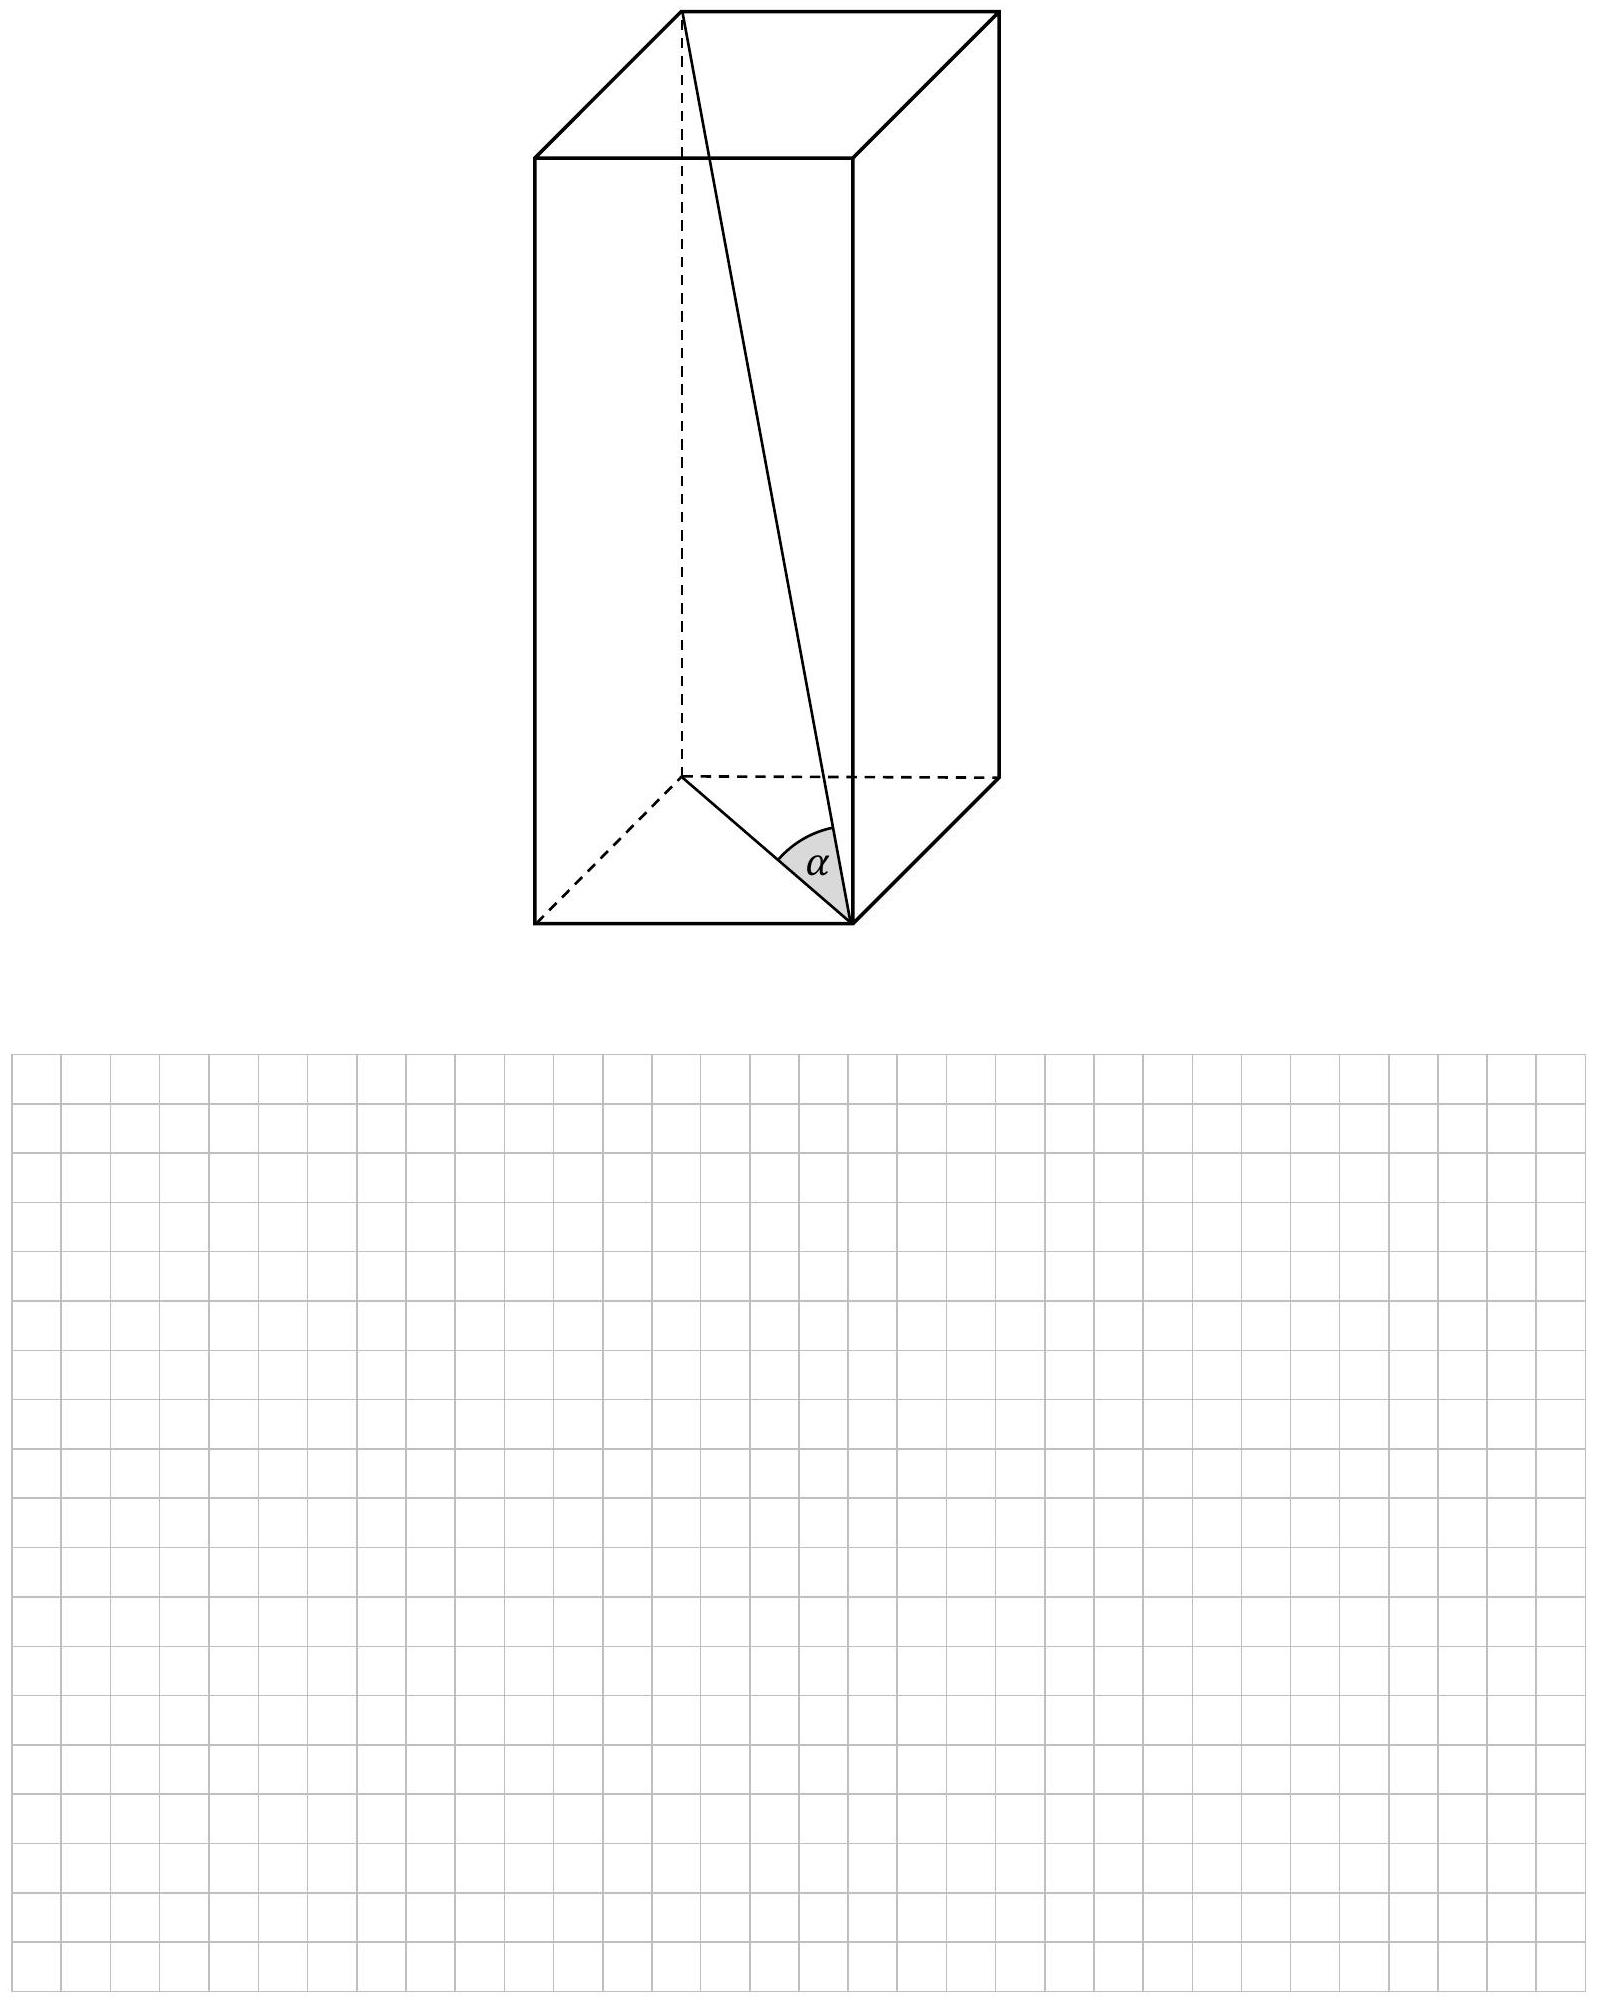
\includegraphics[max width=\textwidth, center]{2024_11_21_0a35d272448d5080a489g-28}\\

\includegraphics[max width=\textwidth, center]{2024_11_21_0a35d272448d5080a489g-29}

\begin{center}
\begin{tabular}{|c|l|c|}
\hline
\multirow{2}{*}{\begin{tabular}{c}
Wypełnia \\
egzaminator \\
\end{tabular}} & Nr zadania & 36. \\
\cline { 2 - 3 }
 & Maks. liczba pkt & 5 \\
\cline { 2 - 3 }
 & Uzyskana liczba pkt &  \\
\hline
\end{tabular}
\end{center}

\section*{BRUDNOPIS (nie podlega ocenie)}

\includegraphics[max width=\textwidth, center]{2024_11_21_0a35d272448d5080a489g-30}\\

\includegraphics[max width=\textwidth, center]{2024_11_21_0a35d272448d5080a489g-31}

\section*{MATEMATYKA}
\section*{Poziom podstawowy}
Formuła 2015

\section*{MATEMATYKA}
Poziom podstawowy Formuła 2015

\section*{MATEMATYKA}
Poziom podstawowy\\
Formula 2015


\end{document}